\chapter{Implementation \label{cha:chapter5}}

This chapter describes the implementation details, including the structural decisions and  encountered development challenges, of the Rollup System based on the system described at \ref{sec:2_adspProject}. Figure \ref{fig:fig:5_drawings-final_rollup_archotecture.png} shows the system's new architecture, clearly distinguishing Layer 1 and Layer 1 components and showing the interactions between them.

\begin{figure}[ht]
	\centering
	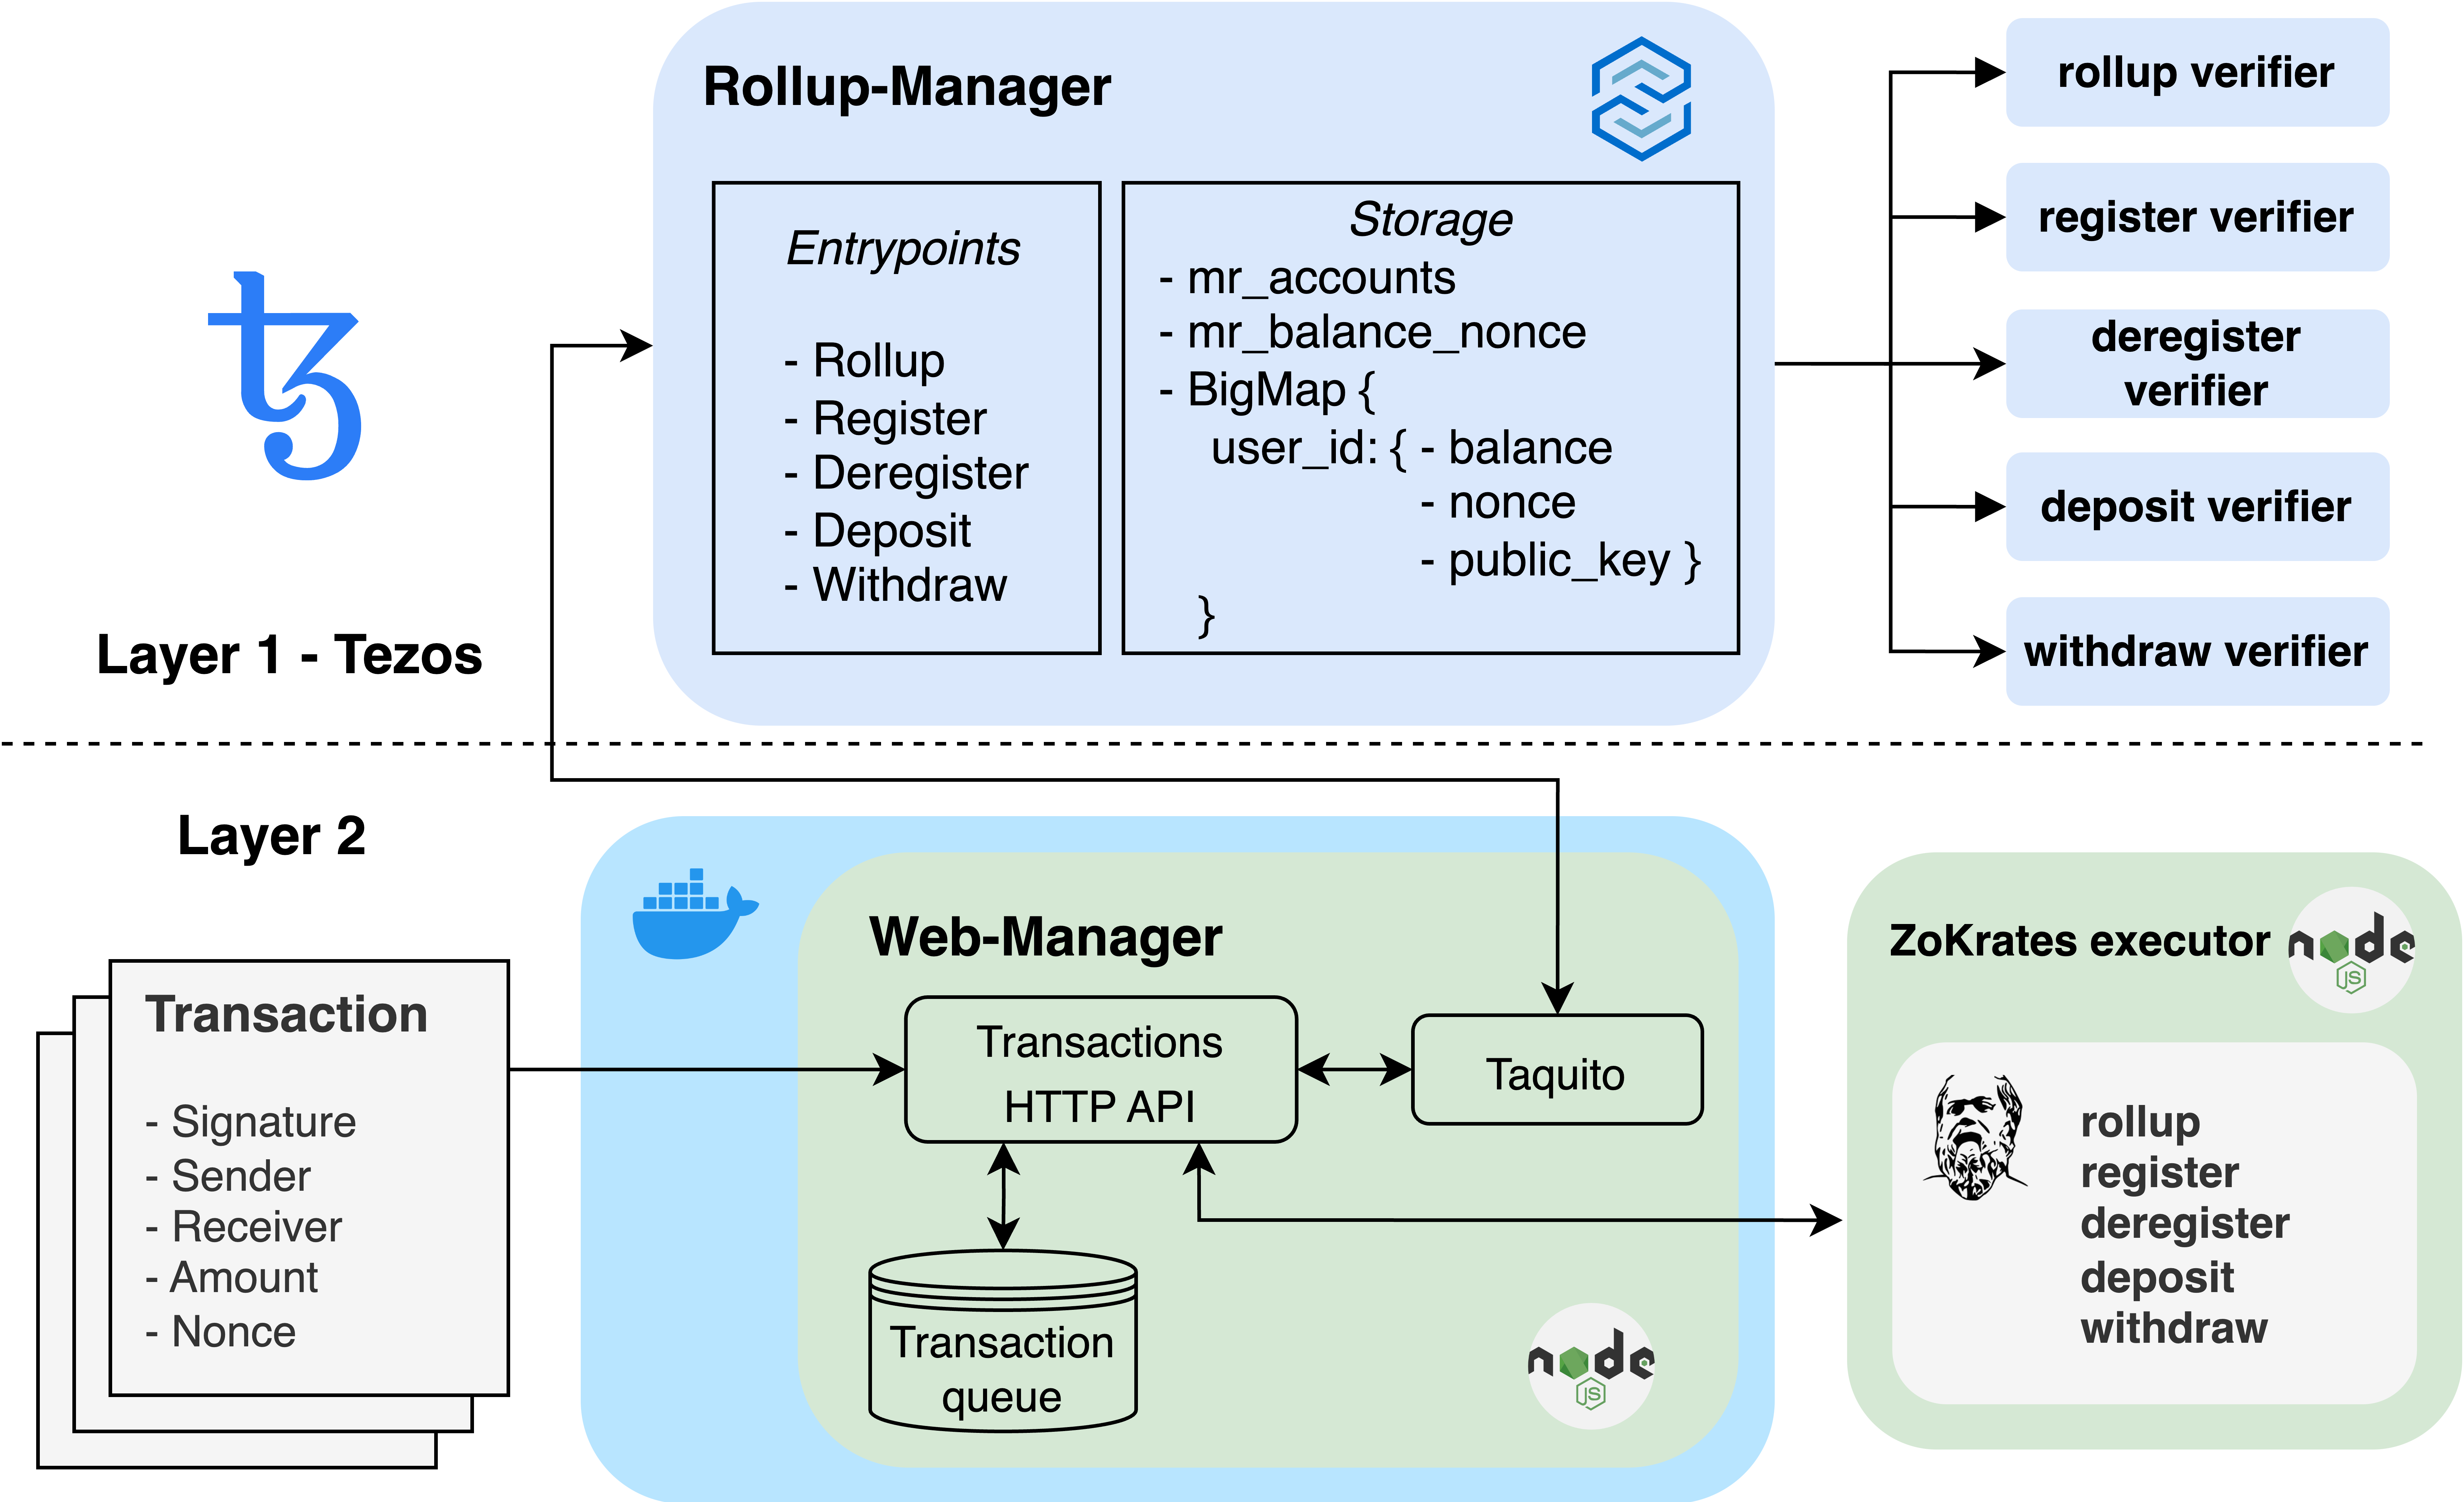
\includegraphics[width=0.9\columnwidth]{5_drawings-final_rollup_architecture.png}
	\caption[Scaling Solutions]{Architecture of the Rollup System.}  
	\label{fig:fig:5_drawings-final_rollup_archotecture.png}
  \end{figure} 

\section{Technologies\label{sec:technologies}}

The blockchain components are constructed utilizing the Tezos blockchain\footnote{\url{https://tezos.com/}} and the SmartPy\footnote{\url{https://smartpy.io/}} smart contract language. The Rollup System is deployed on the Tezos Ghostnet test network.

To engineer the Layer 2 components, web servers are developed using nodejs and Typescript running in Docker containers. The implementation of Rollup programs is accomplished through the utilization of the ZoKrates toolbox\footnote{\url{https://github.com/ZoKrates/ZoKrates}}, a comprehensive zk-SNARKs toolkit designed to facilitate the creation of verifiable computation programs.

The interaction between the Layer 2 and Layer 1 is made possible through the utilization of the Taquito\footnote{\url{https://tezostaquito.io/}} library, a TypeScript library that provides a simple interface for interacting with the Tezos blockchain.

Those technologies were already decided at the time of the project's inception, as they were the most suitable for the project's objectives. The Tezos blockchain was chosen due to its easy development and deployment, as well as the missing Layer 2 solutions.
\todo[inline]{Write why ZoKrates was chosen}

\section{Repeated Transactions Attack}
\label{sec:repeatedtransactionsattack}

To mitigate the risk of an attacker initiating repeated transactions, the nonce mechanism comes into play: each account holds a nonce, stored on Layer 1. When a transaction is submitted, it must include a nonce incremented by one, thereby facilitating the validation of transaction execution history.

Within the ZoKrates environment, proving the usage of updated balances and nonces necessitates computation of a merkle tree for the provided balance and nonce lists. This implies calculating two full binary trees, thereby increasing complexity. A workaround involves concatenating and hashing balances and nonces for individual users, forming a single merkle tree of these concatenated values. This approach incurs only the complexity of the concatenation function, involving a number of hashes equivalent to the number of accounts, ultimately substantiating the updated balances and nonces.

Changes were introduced to the rollup execution to incorporate the computation of new nonces alongside new balances. It's essential that ZoKrates receives transactions ordered by nonce for each user. While transactions from diverse users can be received, those from a single user must be ordered by nonce. The algorithm for verifying transaction nonces and calculating new nonces is as follows:
\begin{itemize}
	\item Initialize \textit{nonce\_array} and \textit{balance\_array}, with the current nonces and balances of all users;
	\item Iterate through the transactions:
	\begin{itemize}
		\item Check in \textit{nonce\_array} if the transaction nonce equals the sender's nonce plus one;
		\item If true:
		\begin{itemize}
			\item Increment senders's nonce in array \textit{nonce\_array};
			\item Decrement sender's balance in array \textit{balance\_array};
			\item Increment receiver's balance in array \textit{balance\_array};
			\item Proceed to next transaction;
		\end{itemize}
		\item If false:
		\begin{itemize}
			\item Fail program execution.
		\end{itemize}
    \end{itemize}
\end{itemize}

This approach accommodates multiple transactions from the same user, thwarting duplicate transaction execution.

The rollup execution complexity experiences minimal augmentation, as the nonce check coincides with balance calculation in the same loop, facilitating direct array access and preserving an O(n) complexity.

\section{Hash Function}

Hash functions play a crucial role in the Rollup execution process. They are extensively used for various tasks such as creating Merkle Trees, concatenating balances and nonces, and verifying signatures. One widely supported hashing function in this context is SHA-256. The initial implementation of the Rollup system employed the SHA-256 function provided by the ZoKrates toolbox. However, as demonstrated in Section \ref{subsec:6_hashfunc}, the use of this function introduces a significant number of constraints to the compiled Zokrates program, resulting in exponential complexity during execution. This inefficiency arises from the fact that classical cryptographic schemes predominantly consist of boolean operations, which become inefficient within a ZK-SNARK circuit \cite{belles-munoz_twisted_2021}.

A more recent hash function, known as Poseidon \cite{grassi_poseidon_nodate}, has been developed with a specific focus on efficiency within zk-SNARK circuits. By transitioning the Rollup system's hash function from SHA-256 to Poseidon, the number of constraints added to the program has been reduced by a factor of 100.

Notably, the adoption of the Poseidon hash function necessitates a revision of the system storage. While SHA-256 operates on 256-bit blocks, Poseidon operates on field sizes defined by the underlying elliptic curve. Additionally, considering the process of signature verification, the payload of a signed message must be hashed to fit a predetermined size prior to verification. In the case of Zokrates signature verification, which expects 512 bits of data, padding must be added after hashing the payload with Poseidon. This is due to the fact that the bls12\_381 curve on ZoKrates operates on a 254-bit field size. To meet the expected size, a padding of 258 bits, filled with zeros, is appended to the right of the payload's hash.

\section{Proof Reduction and Compression}
When creating ZoKrates' private and verification keys it is important to note that the size of the keys is proportional to the number of outputs that the ZoKrates program has. When executing a Rollup the outputs are the new Merkle Tree of the concatenated balances and nonces, plus the list of balances and nonces. Those values are in fact used to update the internal state on the Smart Contract living in Layer 1. As described in \ref{sec:3_smartContractsRequirements} the whole operation sent to the blockchain must not exceed 32768 bytes. Section \ref{subsec:6_verifierproofsize} shows how the proof size increases out of control when the number of users increases. This leads to the impossibility of sending the proof to the Rollup Smart Contract, making the system unusable. A proposed solution consists of realizing a reduction and compression of the outputs of the zokrates program.

\subsection{Proof Size Reduction}

To achieve a reduction in the number of outputs from the ZoKrates program, a change is made in the program's logic. Instead of returning the entire list of balances and nonces, the program only returns the altered balances and nonces. This adjustment introduces the requirement for an index that can be used to identify users in the list.

For every transaction, certain information needs to be returned: the sender's index, balance, and nonce, as well as the receiver's index and balance. In a hypothetical rollup system with 4096 users and 128 transactions per rollup, the outputs of the ZoKrates program shrink from 8193 to 641 (inclusive of the Merkle Root). This reduction significantly cuts down the proof size. Notably, in a Rollup system, many users remain inactive, participating infrequently in the rollup. This dynamic creates a considerable gap between the registered user count and the number of transactions, which enables this mechanism.

Furthermore, this approach proves more advantageous when a single user initiates multiple transactions to the same recipient, as the sender's index and balance are only returned once.

\subsection{Proof Compression}

ZoKrates allows operating on fields of size 254 bits. The proof itself is made up of entries in these fields, no matter the original type of value. Even a simple boolean or a 254-bit value gets represented using just one field entry. This applies to lists of changed indexes, balances, and nonces too. When returning the list of modified indexes, balances and nonces they will occupy a single field value for just 32 bit of information.

By combining indexes, balances, and nonces into one field value, we can fit more info in a single entry. This merging cuts down the number of field entries from the ZoKrates program, which in turn shrinks the proof size. Here's a snippet of how this compression works within the ZoKrates program:

\begin{lstlisting}[language=C++]
field[NUM_TRANSACTIONS] mut result = [0; NUM_TRANSACTIONS];
for u32 i in 0..NUM_TRANSACTIONS {
  // Calculate new balances and nonce
  ......
  // Compress indexes, balances, and nonces
  bool[32] index_send_bits = u32_to_bits(index_sender);
  bool[32] balance_send_bits = u32_to_bits(balance_sender);
  bool[32] nonce_send_bits = u32_to_bits(nonce_sender);
  bool[32] index_rec_bits = u32_to_bits(index_receiver);
  bool[32] balance_rec_bits = u32_to_bits(balance_receiver);
  bool[254] joined = [
    ...index_send_bits, ...balance_send_bits,
    ...nonce_send_bits, ...[false; 94],
    ...index_rec_bits, ...balance_rec_bits
  ];
  result[i] = pack(joined);
}
\end{lstlisting}

This process returns one field value for each transaction. The first 96 bits hold sender-related data, followed by a 94-bit padding, and then 64 bits for receiver-related data.

Another way to improve this is by concatenating all data into one bit array, and then taking 254-bit chunks from it to create field values.

To get back the original values, the Smart Contract needs to decompress the data. At the moment, the ability to get data from field values as bytes is there, but the current SmartPy version lacks converting from Bytes to Nat. When that feature comes in, it wil be possible to restore original values from field values. The upcoming benchmarks will also account for the estimated cost of this value conversion.

\section{Storage}

Initially, the storage was designed with the intention of accommodating a limited number of users, employing a standard Map. Standard maps in Tezos are always deserialized at every contract execution, even if the elements of the map will not be used. This approach is suitable for debugging or where there is the need of iterating through the entire map without knowing its size. 

With scalability as a focal point, the storage structure was updated to handle a growing user base through the adoption of a Big Map. This change is pivotal, due that the Big Map is lazily deserialized\footnote{\url{https://tezos.gitlab.io/michelson-reference/\#type-big_map}}, avoiding the waste of gas during contract calls to deserialize the entire accounts Map. It is, in fact, a dangerous issue, as the gas limit could be reached before the contract is deserialized, making it unusable as described in \ref{subsec:gasLimit}.

\section{ZoKrates Native Execution}
The execution of ZoKrates programs demands substantial resources, as evidenced in Section \ref{sec:benchmarks}. As a consequence, executing ZoKrates programs is allocated to a distinct server. This server operates as an independent entity, called upon by Web-Manager. This strategy serves the dual purpose of optimizing resource allocation and facilitating scalability. Specifically, the architecture enables the isolation of resource-intensive tasks to a separate server, allowing efficient utilization and the ability to scale individual components as needed.

The primary web server dispatches requests, including the needed inputs fetched from the Manager smart contract, to the ZoKrates servers. These dedicated servers execute the ZoKrates programs, returning the results to the primary server. Notably, the utilization of a containerized environment for the ZoKrates server introduces challenges. The approach of running ZoKrates programs directly on the machine is chosen to mitigate the introduction of overhead stemming from OS-level virtualization, particularly relevant in scenarios involving pre-existing virtualized environments, such as cloud computing contexts.

\section{New Features Implementation}
This section details the implementation of the new features of the project, including the problems encountered and the solutions devised.

\subsection{Registration and Deregistration}

This segment elucidates the registration and deregistration procedures for users. The primary objective is to add and remove users from storage, creating empty user entries during deregistration. This approach maintains user positioning within storage, allowing utilization of existing indexes.

Tezos supports optional types, enabling a value to be set as None, indicating its absence. This feature proves valuable during user removal from storage. The new storage Big Map, representing registered users, now comprises:
\begin{itemize}
	\item \textbf{index}: A natural number representing the user's index within storage;
	\item \textbf{mutez balance}: The user's balance;
	\item \textbf{nonce}: The user's nonce;
	\item \textit{optional} \textbf{public key}: The user's public key.
\end{itemize}

Given the resource-intensive nature of merkle tree generation, registration and deregistration processes are executed within dedicated ZoKrates programs and not in the smart contracts.

\subsubsection{Registration\label{subsec:registration}}

To register a new user, the two Merkle Trees must be recomputed, integrating the new user's public key, balance, and nonce. A ZoKrates program performs this computation, returning the new root hashes of both Merkle Trees. These hashes are then used by the manager smart contract to update the storage, incorporating new roots and the new user. The ZoKrates program requires the precise position for inserting the new user's data. This position is determined externally by a manager, which can communicate with an RPC to ascertain the first vacant slot within the storage's Big Map. The registration process verifies if the designated position holds an account with an empty key, balance, and nonce set to zero. Subsequently, the user's nonce is set to one, balance to zero, and public key to the user's public key.

\subsubsection{Deregistration}

Deregistration closely mirrors the registration process outlined in Section \ref{subsec:registration}. The ZoKrates deregistration program takes the user's index to be deregistered, along with other standard inputs. This program sets the user's public key to None, balance to zero, and nonce to zero. The updated root hashes of both Merkle Trees are returned by the deregistration program. The manager contract then employs these new roots to update storage, removing the user entry at the specified index.

\subsection{Deposit\label{subsec:deposit}}
The deposit process into the Layer 2 system is intricate due to the requirement of recalculating the merkle tree involving balances and nonces. As a result, the deposit procedure is divided into two distinct phases: the initial phase entails transferring funds from the user's account to the manager smart contract via a dedicated entrypoint call in the contract; the subsequent phase involves executing a ZoKrates program to recompute the merkle tree of balances and nonces, ultimately producing the new root of the tree. Figure \ref{fig:5_drawings-sequence_deposit.png} illustrates the deposit process.

\subsubsection{Phase 1: Transferring Funds to Manager Contract}
The deposit process is instigated by the user, who invokes the \textit{deposit} entrypoint within the manager contract and specifies the index of the account within the user Big Map. Subsequently, the manager contract facilitates the transfer of the designated sum from the user's account to its own account. Additionally, an internal record of pending deposits is maintained.

This internal deposit record adopts the structure of a \textit{Map (nat mutez)}, where the key corresponds to the user's index in the user Big Map, and the value signifies the sum of funds intended for deposition. This configuration accommodates the acceptance of multiple deposits from a single user, effectively tracking the specified deposit amounts.

In the aftermath of the first phase, the user remains unable to expend the transferred sum until the conclusion of the second phase.

\subsubsection{Phase 2: Merkle Tree Recalculation}
The second phase is initiated by a Web Server that detects a considerable accumulation of deposits in the deposit queue. Subsequently, the Web Server accesses the deposit list and initiates the ZoKrates program responsible for recalculating the merkle tree inclusive of the new deposits. Following this computation, the Web Server calls the \textit{receive\_deposit\_proof} entrypoint within the manager contract, providing the freshly computed merkle tree root as a parameter. Consequently, the manager contract updates the root of the merkle tree associated with balances and nonces, adjusts user balances to incorporate the deposited funds, and ultimately eradicates the deposits from the internal pending deposit list.

\begin{figure}[ht]
	\centering
	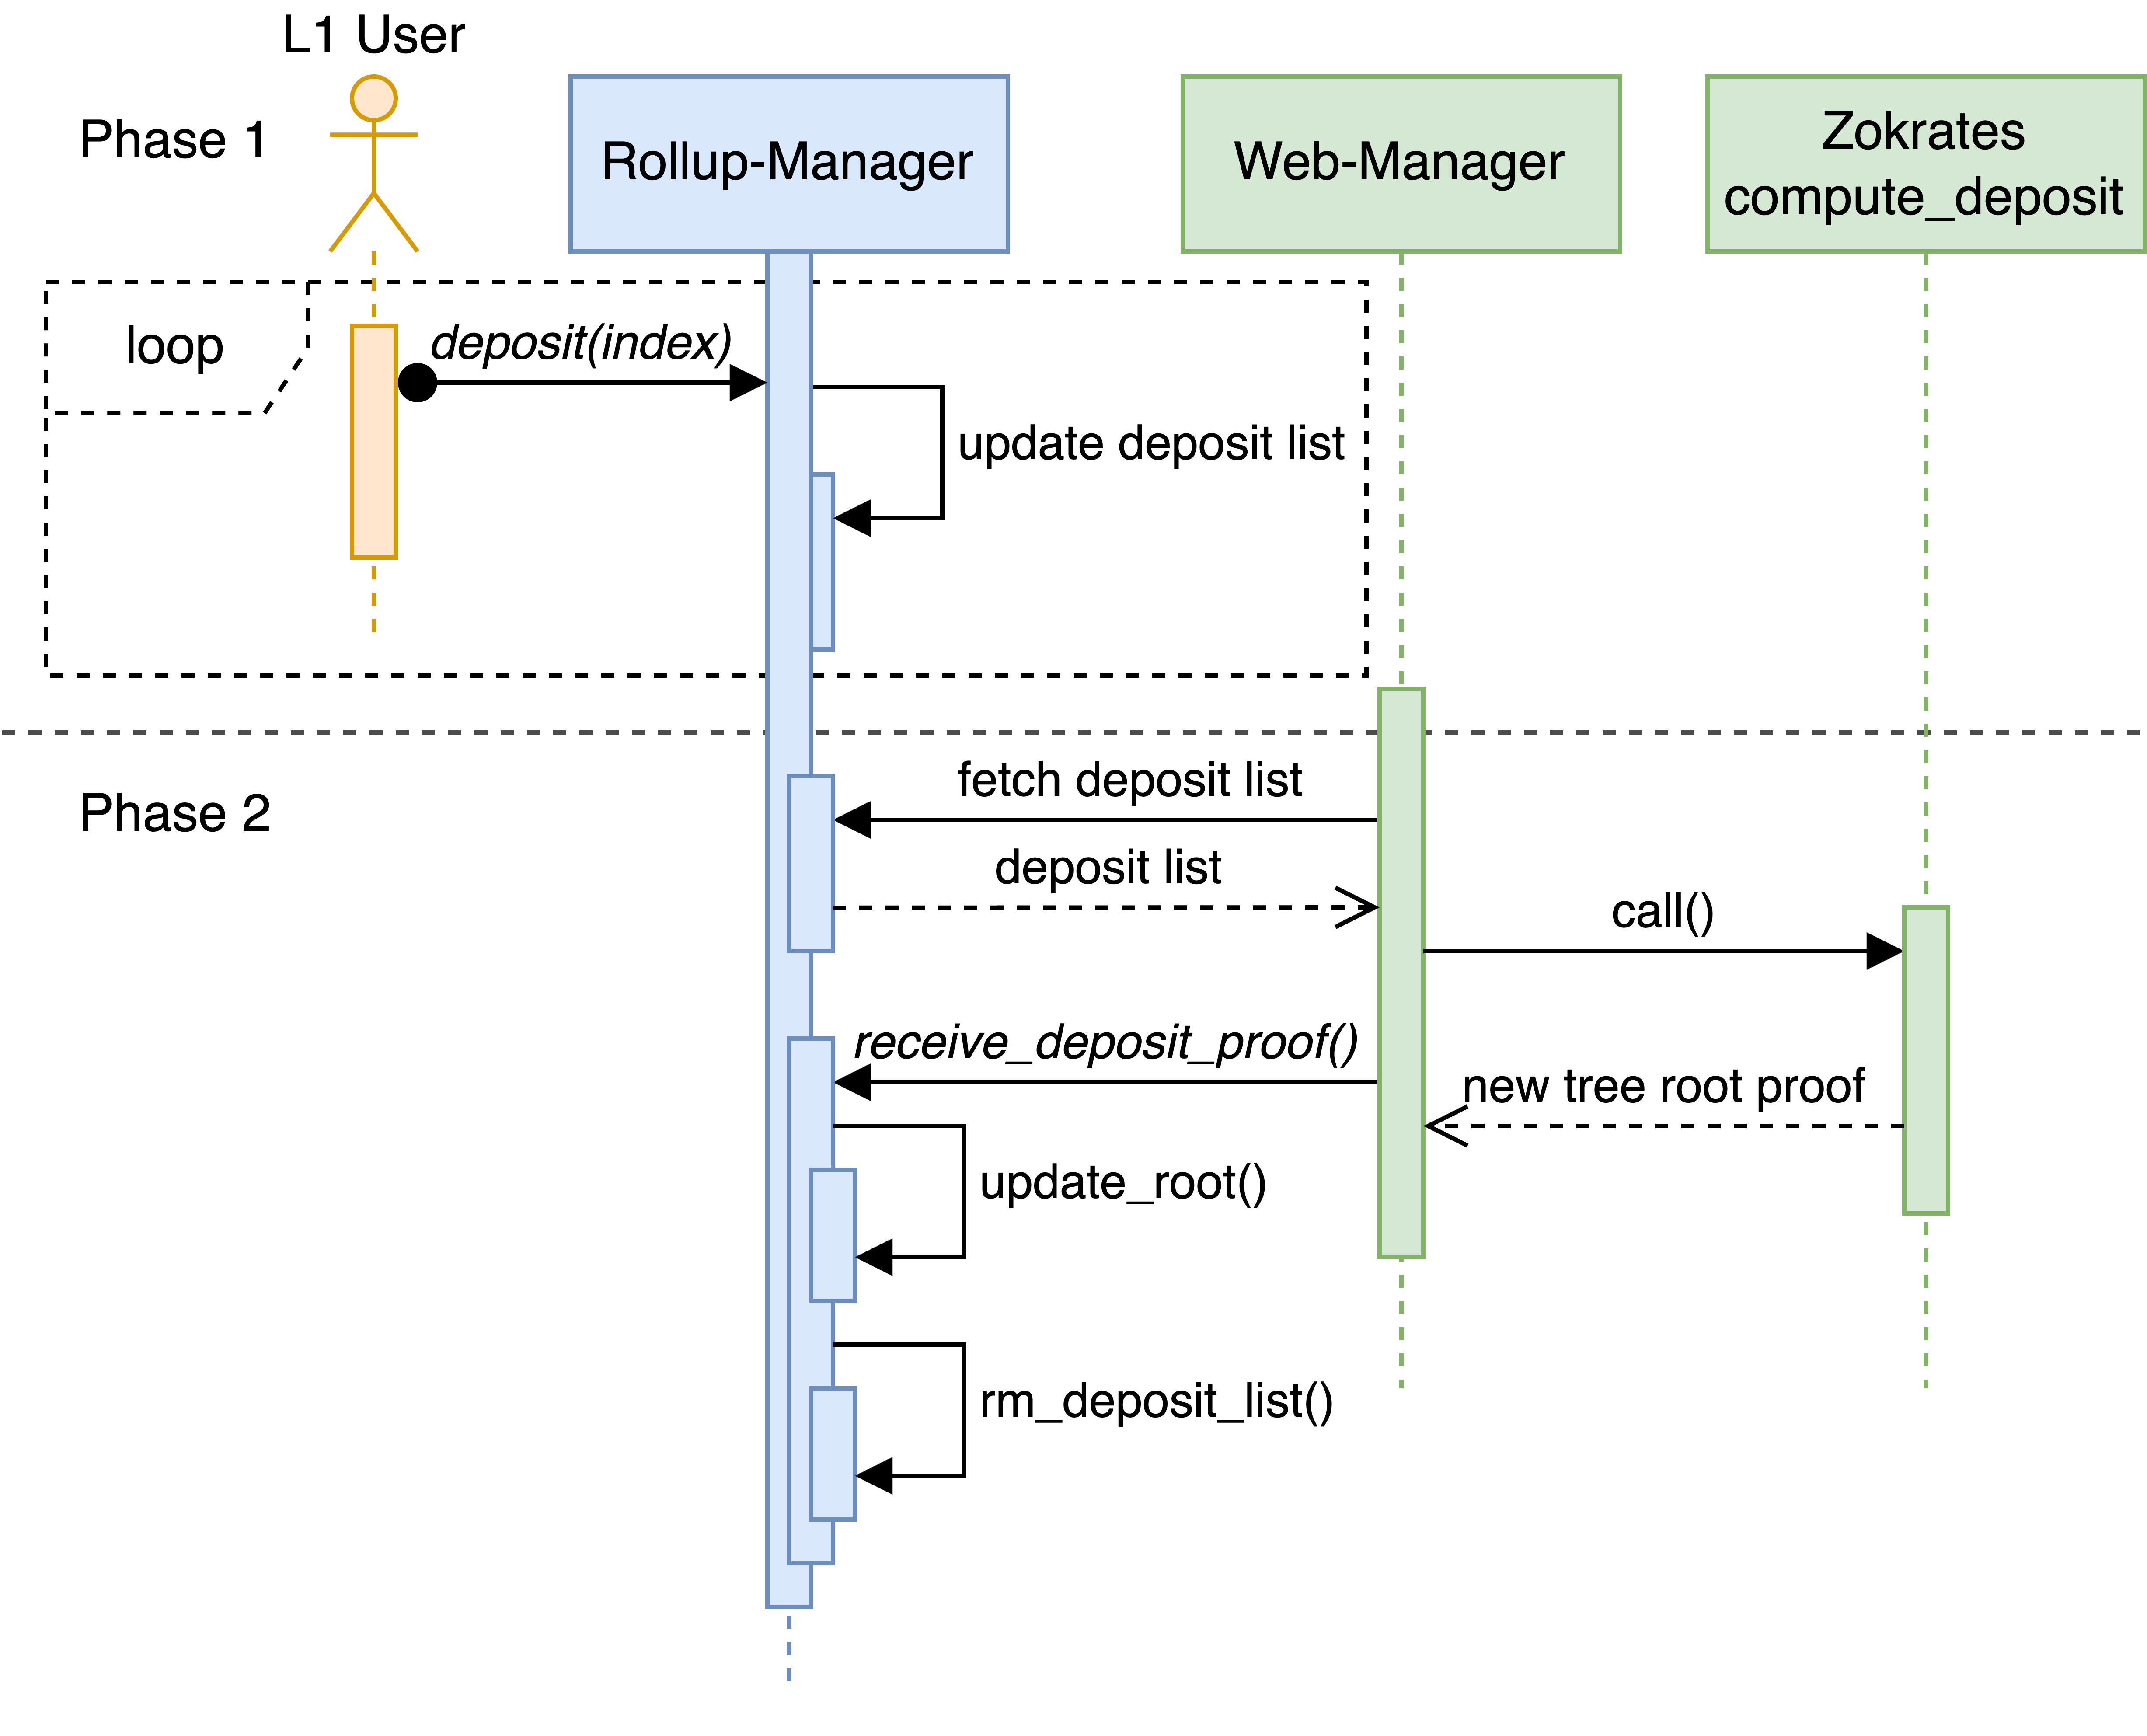
\includegraphics[width=0.7\columnwidth]{5_drawings-sequence_deposit.png}
	\caption[Scaling Solutions]{Sequence Diagram of Deposit Process}  
	\label{fig:5_drawings-sequence_deposit.png}
  \end{figure} 

  \subsection{Withdraw}
  This section delineates the Withdrawal process, enabling the movement of funds from the Layer 2 system to the Layer 1 system. The withdrawal process diverges from the deposit process expounded in Section \ref{subsec:deposit}. Notably, withdrawals operate within a single phase, a strategic choice that expedites the withdrawal procedure, affording users the prompt retrieval of their funds without the necessity of reaching a threshold of users in the withdrawal queue.
  
  The withdrawal initiation commences as users dispatch withdrawal requests to the Web Server. Subsequently, the Web Server retrieves the user's balance and nonce from the manager contract and generates withdrawal inputs for the dedicated ZoKrates program. This ZoKrates program orchestrates the computation of the new root hash for the merkle tree containing balances and nonces. This computation involves the subtraction of the user-specified amount. The computed new root hash is then relayed back to the Web Server. In turn, the Web Server invokes the \textit{receive\_withdrawal\_proof} entrypoint within the manager smart contract. This invocation encompasses the provision of the new root hash as a parameter.
  
  Within the manager contract, the merkle tree root hash undergoes an update, alongside adjustments to the user's balance and nonce. Subsequently, the requested sum is transferred to the user's account, finalizing the withdrawal process.
